\section{Method Overview}
\label{sec:method}
In this section, we introduce our formulation of the joint registration and co-segmentation problem for point sets. Tabel~\ref{tab:symbol} lists all the symbols used in our formulation. The input of our problem is a group of 3D point sets  $\mathcal{V}=\{\mathbf{V}_m\}^{M}_{m=1}$ that are captured at $M$ different times in a scene, where objects move in different ways. Each point set $\mathbf{V}_m=\{\pmb{v}_{mi}\}^{L_m}_{i=1}$ contains $L_m$ 3D points. Our problem is to simultaneously partition the point sets into $N$ objects and figure out the transformations from objects to each point set. For partitioning, we output point-wise label vectors $\{\pmb{y}_m\}$ for each input point set to indicate its object partition. For registration, we output $\{\mathbf{R}_{mn},\pmb{t}_{mn}\}$ to indicate the transformations from $N$ different objects to $M$ different point sets.
\begin{table}[!hbp]
\centering
\caption{Table of symbols used in the paper.} 
\label{tab:symbol}
\begin{tabular}{c|l}
\hline
Symbol         & Definition\\
\hline
$M$            & The number of input point sets.\\
$\mathbf{V}_m$ & The $m^{th}$ input point set.\\
$\mathcal{V}$  & The input point sets $\{\mathbf{V}_m\}^{M}_{m=1}$.\\
$L_m$          & The number of points of the $m^{th}$ point set $\mathbf{V}_m$.\\
$\pmb{v}_{mi}$ & The $i^{th}$ point of $\mathbf{V}_m$.\\
$\pmb f_{mi}$   & The point-wise feature vector of $\pmb v_{mi}$.\\
$z_{mi}$       & The latent parameter for $\pmb v_{mi}$.\\
               & $z_{mi}=k$ means $\pmb{v}_{mi}$ is generated by $k^{th}$ Gaussian. \\
$\mathcal{Z}$            & $\mathcal{Z}=\{z_{mi}|m=1...M,i=1...L_m\}$.\\
$N$            & The number of objects in the scene.\\
$K_n$          & The number of Gaussian models for the $n^{th}$ object. \\
$K_S$		   & The sum of $\{K_1,K_2,\cdots,K_{n-1}\}$\\
			   & $K_S = \sum_{i=1}^{n-1}K_i$\\
$K_{all}$      & The total number of Gaussian models of all objects. \\
               & $K_{all} = \sum_{n=1}^N K_n $.\\
$p_k$          & The weight of $k^{th}$ Gaussian. $\sum_{k=1}^{K_{all}}p_k=1$.\\
$\pmb x_k$     & The centroid of $k^{th}$ Gaussian model.\\
$\pmb {x}^{v}_k$   & The centroid of $k^{th}$ Gaussian for point position.\\
$\pmb {x}^{f}_k$   & The centroid of $k^{th}$ Gaussian for point feature.\\
$\Sigma_k$     & The covariance matrix of $k^{th}$ Gaussian model.\\
$\sigma_k$     & $\Sigma_k=\sigma_k^2\mathbf{I}$, where $\mathbf{I}$ is an identity matrix.\\
$\sigma^v_k$   & Gaussian covariance parameter for point position\\
$\sigma^f_k$   & Gaussian covariance parameter for point feature\\
$\phi_{mn}$    & Rigid transformation from object $\mathbf{O}_n$ to point set $\mathbf{V}_m$.\\
%$\mathbf{R}_{mn}$ & The rotation matrix for $\phi_{mn}$.\\
%$\mathbf{t}_{mn}$ & The translation vector for $\phi_{mn}$.
\hline
\end{tabular}
\end{table}
\subsection{Basic Formulation}
For robustness, we do not model the point sets as a simple composition of transformed 3D points in each object model. Instead, we model the point sets as realizations of an unknown central Gaussian mixture model (GMM) from of the transformed object models. In other words, we explicitly separate total $K_{all}$ Gaussian models to $N$ groups to represent $N$ objects $\{\mathbf{O}_n\}_{n=1}^N$ as
\begin{equation}
\begin{aligned}
\{
\underbrace{ \{\pmb{x}_{1},\Sigma_{1}\}, \cdots, \{\pmb{x}_{K_1},\Sigma_{K_1}\}  }_{\mathbf{O}_1},&\underbrace{ \{\pmb{x}_{K_1+1},\Sigma_{K_1+1}\}, \cdots, \{\pmb{x}_{K_1+K_2},\Sigma_{K_1+K_2}\}  }_{\mathbf{O}_2},\\ 
\cdots \cdots,& 
\underbrace{ \{\pmb{x}_{K_S+1},\Sigma_{K_S+1}\},\cdots,\{\pmb{x}_{K_S+K_n},\Sigma_{K_S+K_n}\}  }_{\mathbf{O}_n},\cdots \}
\end{aligned}
\end{equation}
where $K_S = \sum_{i=1}^{n-1}K_i$.

The Gaussian centroids $\{\pmb{x}_{k}\}$ represent the point positions in objects. $\{\Sigma_{k}\}$ qautify the variance of point positions in objects. $\mathbf{O}_n$ has $K_n$ Gaussian models and $\{K_n\}_{n=1}^N$ are predefined.
Each object model $\mathbf{O}_{n}$ is rigidly transformed to each point set $\mathbf{V}_m$ with a transformation $\phi_{mn}(\pmb{x}_{k})=\mathbf{R}_{mn}\pmb{x}_{k}+\pmb{t}_{mn}$ for $\pmb{x}_{k} \in \mathbf{O}_n$
%
Hence, for each point $\pmb{v}_{mi}$ in a point set $\mathbf{V}_m$, given object models $\{\mathbf{O}_{n}\}$ and their rigid transformations $\{\phi_{mn}\}$ to the point sets, we can write
\begin{equation}
\label{equ:model}
P(\pmb{v}_{mi})=\sum^{K_{all}}_{k=1}p_k\mathcal{N}(\pmb{v}_{mi}|\phi_{mn}(\pmb{x}_k),\Sigma_k)
\end{equation}
which treat the $i^{th}$ observed point $\pmb{v}_{mi}$ from the $m^{th}$ point set as a sample point generated by a large Gaussian mixture model that represent $N$ objects all together.

Given the generative representation of point sets, the unknown model parameters of our joint registration and segmentation problem are
%
\begin{equation}
\varTheta=\big \{\{p_k,\pmb{x}_{k},\Sigma_k\}_{k=1}^{K_{all}},\{\phi_{mn}\}_{m=1,n=1}^{M,N}, \{\pmb{y}_{m}\}^{M}_{m=1}\big\}.
\end{equation}
 
To estimate the parameters $\Theta$ to fit all the input point sets Without knowing object labels for all 3D points, the problem can be solved in the EM framework of Expectation-Maximization. 
%
In particular, we bring in hidden variables as: 
\begin{equation}
\mathcal{Z}=\{z_{mi}|m=1...M,i=1...L_m\},
\end{equation}
%
such that $z_{mi}=k(k=1,2...,K_{all})$ assigns the observed point $\pmb{v}_{mi}$ to the $k^{th}$ component of the Gaussian mixture model. 
%
We aim to maximize the expected complete-data log-likelihood:
\begin{equation}
\label{equ:obj0}
\mathcal{E}(\Theta|\mathcal{V},\mathcal{Z})=\mathbb{E}_{\mathcal{Z}}[\ln P(\mathcal{V},\mathcal{Z};\Theta)|\defV]={\sum_{\mathcal{Z}}P(\defZ|\defV,\Theta)\ln{P(\mathcal{V},\mathcal{Z};\Theta)}}.
\end{equation}


This formulation can be seen as an adaption of the joint registration formulation in \cite{Evangelidis2014}, upon which we separate Gaussian models into groups to express multiple objects. 
%
The latent parameter $\defZ$ that assigns observed points to Gaussian models can naturally indicate the object level segmentation.
%
Under the assumption that the input points are independent and identically distributed, we can rewrite the objective defined in Eq.~(\ref{equ:obj0}) into:
%
\begin{equation} \label{equ:obj2}
\Theta=\arg\max\sum_{mik}\alpha_{mik}(\ln p_k + \ln P(\pmb{v}_{mi}|z_{mi}=k;\Theta)),
\end{equation}
%
where $\alpha_{mik} = P( z_{mi} = k | \pmb{v}_{mi} ; \Theta )$.


By bringing in Eq.~\ref{equ:model} and ignoring constant terms, we can rewrite the objective as:
\begin{equation}
\label{equ:obj3}
\Theta=\arg\max\sum_{mik}\alpha_{mik}(||\pmb{v}_{mi}-\phi_{mn}(\pmb{x}_k)||_{\Sigma_k}^2 + \ln |\Sigma_k| - 2\ln p_k), 
\end{equation}
%
where the $|\cdot|$ denotes the determinant and $||\pmb{x}||_{\mathbf{A}}^2= \pmb{x}^T\mathbf{A}^{-1}\pmb{x}$. 
%
It is predefined that $\pmb{x}_k$ is one of the Gaussian centroids used to represent $n^{th}$ object, which is why we apply transformation $\phi_{mn}$ on to the $\pmb{x}_k$. 
%
For the convenience of computation, we restrict the model to isotropic covariances, i.e.,$\Sigma_k=\sigma^2\mathbf{I}$ and $\mathbf{I}$ is the identity matrix.
%
Now, we can optimize this through iterating between estimating $\alpha_{mik}$ (Expectation-step) and maximizing $\mathcal{E}(\Theta|\defV,\defZ)$ sequentially with respect to each parameters in $\Theta$ (Maximization-steps).

%These steps are:
\noindent\textbf{E-step}:
this step estimates the posterior probability $\alpha_{mik}$ of $\pmb v_{mi}$ to be a point generated by the $k^{th}$ Gaussian model.
%
\begin{equation}
\label{equ:estep}
\alpha_{mik}=\frac{p_k\sigma_k^{-3}exp(-\frac{1}{2\sigma_k^2}||\pmb v_{mi}-\phi_{mn}(\pmb x_k)||^2)}{\sum_s^{K_{all}}p_s\sigma_s^{-3}exp(-\frac{1}{2\sigma_s^2}||\pmb v_{mi}-\phi_{mn}(\pmb x_s)||^2)}
\end{equation}
%


\noindent\textbf{M-step-a}: this step updates the transformations $\phi_{mn}$ that maximize $\mathcal{E}(\Theta)$, given instant values for $\alpha_{mik}$, $\pmb{x}_k$, $\sigma_k$.
%
We only consider rigid transformations, making  $\phi_{mn}(\pmb{x})=\mathbf{R}_{mn}\pmb{x}+\mathbf{t}_{mn}$. The maximizer $\mathbf{R}_{mn}^*,\mathbf{t}_{mn}^*$ of $\mathcal{E}(\Theta)$ is the same with the minimizers of the following constrained optimization problems
%
\begin{equation}
\left\{
\begin{array}{rcl}
\min_{\mathbf{R}_{mn},\pmb{t}_{mn}}&      &||(\mathbf{W}_{mn}-\mathbf{R}_{mn}\mathbf{X}_n-\pmb t_{mn}\mathbf{e}^T)\Lambda_{mn}||_F^2\\
s.t.&      &\mathbf{R}_{mn}^T\mathbf{R}_{mn}=I, |\mathbf{R}_{mn}|=1\\
\end{array} \right.
\end{equation}
where $\Lambda_{mn}$ is $K_n \times K_n$ diagonal matrix with elements $\lambda_{mnk}=\frac{1}{\sigma_k}\sqrt{\sum_i^{L_{m}}\alpha_{mik}}$,$L_m$ is the number of point for the $m^{th}$ input point set, $\mathbf{X}_n = [\pmb{x}_{K_S+1}, \pmb{x}_{K_S+2},...., \pmb{x}_{K_S+K_n}]$ where $K_S = \sum_{i=1}^{n-1}K_i$ is the matrix stacked by the centroids of gaussian models that are predefined to represent the $n^{th}$ object. $\mathbf{e}^T$ is a vector of ones, $||\cdot||_F$ denotes the Frobenius norm, and $\mathbf{W}_{mn}=[\pmb{w}_{m(K_S+1)},\pmb{w}_{m(K_S+2)},...,\pmb{w}_{mk},...,\pmb{w}_{m(K_S+K_n)}]$ where $K_S = \sum_{i=1}^{n-1}K_i$, in which $\pmb{w}_{mk}$ is a weighted point as
%
\begin{equation}
\pmb{w}_{mk}=\frac{\sum_{i=1}^{L_m}\alpha_{mik} \pmb{v}_{mi}}{\sum_{i=1}^{L_m}\alpha_{mik}}
\end{equation}

This problem has a similar solution with \cite{Evangelidis2014}. 
The only difference is that we are estimating the transformation from Gaussian models to the input point sets instead of the transformation from input point sets to Gaussian models, since there are multiple group of $\pmb{x}_k$ corresponding to multiple objects in our Gaussian models. The optimal can be given by:
%
\begin{equation}
\label{equ:updateR}
\mathbf{R}_{mn}^*=\mathbf{U}_{mn}\mathbf{C}_{mn}\mathbf{V}_{mn}^T
\end{equation}
\begin{equation}
\label{equ:updatet}
\pmb{t}_{mn}^*=\frac{1}{tr(\Lambda_{mn}^2)}(W_{mn}-\mathbf{R}_{mn}X_n)\Lambda_{mn}^2\mathbf{e}
\end{equation}
where $[\mathbf{U}_{mn},\mathbf{S},\mathbf{V}_{mn}]=svd( \mathbf{W}_{mn}\Lambda_{mn}\mathbf{P}_{mn}\Lambda_{mn}\mathbf{X}_{n}^T )$ and $\mathbf{P}_{mn}=I-\frac{\Lambda_{mn}\pmb{e}(\Lambda_{mn}\pmb{e})^T}{(\Lambda_{mn}\pmb{e})^T\Lambda_{mn}\pmb{e}}$, $I$ is identity matrix. $C_{mn}=diag(1,1,|\mathbf{U}_{mn}||\mathbf{V}_{mn}|)$.

\textbf{M-step-b}: this step we update the parameters related to the Gaussian mixture model and the indicating vector for object segmentation 
\begin{equation}
\label{equ:updatexk}
\pmb x_k^*=\frac{\sum_{m=1}^M\sum_{i=1}^{L_m}\alpha_{mik}(\mathbf{R}_{mn}^{-1}\pmb{v}_{mi}-\pmb t_{mn})}{\sum_{m=1}^M\sum_{i=1}^{L_m}\alpha_{mik}}
\end{equation}
where $\pmb{x}_k$ is one of the Gaussian centroids that is predefined to represent the $n^{th}$ object. 
\begin{equation}
\label{equ:updatesigma}
\sigma_k^{*2}=\frac{\sum_{m=1}^M\sum_{i=1}^{L_m}\alpha_{mik}||(\pmb{v}_{mi}-\pmb t_{mn}-\mathbf{R}_{mn}^*\pmb x_k^*)||_2^2}{3\sum_{m=1}^M\sum_{i=1}^{L_m}\alpha_{mik}}
\end{equation}
\begin{equation}
\label{equ:updatepk}
p_k^*=\frac{\sum_{m,i}\alpha_{mik}}{M}
\end{equation}
\begin{equation}
\label{equ:updatey}
y_{mi}^*=\arg \max_n \sum_{k=\sum_{s=1}^{n-1}K_S+1}^{\sum_{s=1}^{n}K_S} \alpha_{mik} 
\end{equation}
where $y_{mi}$ is the $i^{th}$ entry of the indicate vector $\pmb{y}_{m}$ and it assigns the $i^{th}$ point of $m^{th}$ point set to one of $N$ objects.  
\subsection{Bilateral Formulation}
When considering point-wise features, we can add bilateral terms into the generative model.
\begin{equation}
P(\pmb{v}_{mi},\pmb{f}_{mi})=\sum^{K_{all}}_{k=1}p_k\mathcal{N}(\pmb{v}_{mi}|\phi_{mn}(\pmb{x}^v_k),\sigma v_k)\mathcal{N}(\pmb{f}_{mi}|\pmb{x}^f_k,\sigma^f_k),
\end{equation}
where $\pmb{f}_{mi}$ is the feature vector for point $\pmb{v}_{mi}$ and $\pmb{x}_k^f$ is the feature vector for $k^{th}$ point in object model. As shown in the formulation, there is no transformation applyed onto $\pmb{x}_k^f$, which means that this formulation is only suitable to the features that is rotation and translation invariant. For example, the point color vector(for all the result in this paper we use RGB color as feature vector ) $[red_{mi},green_{mi},blue_{mi}]$ is a suitable feature for this formulation. In this formulation $\mathcal{N}(v_{mi}|\phi_{mn}(xv_k),\sigma v_k)$ is the spatial term and $\mathcal{N}(\pmb{f}_{mi}|\pmb{x}^f_k,\sigma^f_k)$ is the feature term.
For the bilateral formulation, iteration steps will be as follows:

\noindent\textbf{E-step}:in this step the calculation of posterior probability need to consider both the spatial term and the feature term.
\begin{equation}
\label{equ:bestep}
\alpha_{mik}=\frac{p_kP_v( \pmb{v}_{mi},\phi_{mn}(\pmb{x}^v_k),\sigma v_k)P_f(\pmb f_{mi},\pmb x^f_k,\sigma^f_k)}{\sum_s^{K_{all}}p_sP_v( \pmb v_{mi},\phi_{mn}(\pmb{x}^v_s),\sigma^v_s)P_f(\pmb f_{mi},\pmb{x}^f_k,\sigma^f_s)}
\end{equation}
where $P_v(\pmb{x},\pmb{y},\sigma)=\sigma^{-3}exp(-\frac{1}{2\sigma^2}||\pmb{x}-\pmb{y}||^2)$ and $P_f(\pmb{x},\pmb{y},\sigma)=\sigma^{-D(\pmb{x})}exp(-\frac{1}{2\sigma^2}||\pmb{x}-\pmb{y}||^2)$ and $D(\pmb{x})$ means the dimension of the vector $\pmb x$. 

\textbf{M-step-a:}for bilateral formulation, this step is the same with the basic formulation and the update can be done as (\ref{equ:updateR}) and (\ref{equ:updatet}).

\textbf{M-step-b}:for bilateral formulation, this step need not only update model centroids and variance for spatial term as (\ref{equ:updatexk}) and (\ref{equ:updatesigma}).
but also update the centroids and variance for feature term as in (\ref{equ:updatefk}) and (\ref{equ:updatefsigma}).
\begin{equation}
\label{equ:updatefk}
\pmb{x}_k^{f*}=\frac{\sum_{m=1}^M\sum_{i=1}^{L_m}\alpha_{mik}f_{mi}}{\sum_{m=1}^M\sum_{i=1}^{L_m}\alpha_{mik}}
\end{equation}
\begin{equation}
\label{equ:updatefsigma}
\sigma_k^{f*2}=\frac{\sum_{m=1}^M\sum_{i=1}^{L_m}\alpha_{mik}||\pmb f_{mi}-\pmb{x}_k^{f*}||_2^2}{D(f)\sum_{m=1}^M\sum_{i=1}^{L_m}\alpha_{mik}},
\end{equation}
where $D(f)$ is the dimenssion of feature vectors. The update of $p_k$ for bilateral formulation is the same as the basic formulation in Eg.~(\ref{equ:updatepk}).

\subsection{Interaction Design}
\label{sec:imp:interact}
Unfortunately, there are a large number of parameters that can not be easily initialized in our formulation. 
%
In this subsection we first introduce our design of interaction, which is intuitive for users to input the semantic prior this way. We then explain how we can easily initialize those parameters for our optimization based on the manual input.


As demonstrated in Figure~\ref{fig:interact}, we let user choose one of the point sets and place boxes in it to indicate the layout for this point set. From this, we can easily initialize the total number of objects $N$ and determine $\{K_n\}$ which is the numbers of Gaussian mixture models used to represent each object.
\begin{figure}[htb]
	\centering
	\includegraphics[width=.3\linewidth]{images/interact01.png}
	\includegraphics[width=.3\linewidth]{images/interact02.png}
	\includegraphics[width=.3\linewidth]{images/interact03.png}
	\includegraphics[width=.3\linewidth]{images/interact04.png}
	\includegraphics[width=.3\linewidth]{images/interact05.png}
	\includegraphics[width=.3\linewidth]{images/interact06.png}
	\caption{\label{fig:interact}
		From the first to the sixth, the nine images show the procedure of interaction:
		the user pick one point set and place boxes in it to indicate the layout for this point set. The box in white is the box currently under editing. The boxes in other colors are boxes placed to represent object layouts. One color represents one object. The interaction allows multiple boxes to represents same object.(e.g. the desk is represented by three boxes in same color)}
\end{figure}
These two parameters are difficult to be initialized without semantic prior, but with the input of the users we can naturally initialize the $N$ as the number of different color label and the ${K_n}$ as 
\begin{equation}
\label{equ:K_n}
K_n=\frac{V_n}{\sum V_n}K_{all},
\end{equation}
in which the $V_n$ represent the total volume of the boxes in the $n^{th}$ color and the $K_{all}$ is initialized as $K_{all}=\frac{median(L_m)}{2}$ and $\{L_m\}$ are point numbers of $M$ input point sets. This is an empirical choice borrowed from \cite{Evangelidis2014}.\\
%
The expectation maximization framework is easily converged to a local optimal. To cope with this problem we further use this layout (boxes) from interaction as a soft constraint to guide the optimization and constrain the shape of generated object model. Such constraint is enforced by simply altering the posterior probability $\alpha_{mik}$ as
%
\begin{equation}
\label{equ:alteralpha}
\alpha_{mik}^*=\frac{\alpha_{mik}\beta_{mik}}{\sum_{i,k}\alpha_{mik}\beta_{mik}}
\end{equation}
where the $\beta_{mik}$ is the prior probability according to the boxes. It is defined as:
\begin{equation}
\beta_{mik}=\left\{
\begin{array}{rcl}
1& &\pmb v_{mi} \in B_n\\
\exp(-\frac{\min_{\pmb v_{mj}}|| \pmb v_{mi} - \pmb v_{mj} ||_2^2  )}{L})& &\pmb v_{mi} \notin B_n~and~\pmb v_{mj} \in B_n\\
\end{array} \right.
\end{equation}
where the $B_n$ is a point set that is enclosed by the boxes used to represent the layout of $n^{th}$ object. The $k^{th}$ Gaussian model is predefined to be one of the Gaussians used to represent $n^{th}$ object. $\min_{v_{mj}}|| v_{mi} - v_{mj} ||_2^2$ is actually the squared euclidean distance from point $v_{mi}$ to the point set $B_n$, as we define the distance from a point to a point set as the minimum distance from the point to any point inside the point set. $L$ here is a constant number with $L=2r^2$, and $r$ is the median of the radius of input point sets. The radius of a point set is half of length of diagonal line of its axis-aligned bounding box.   
\begin{figure}[htb]
	\centering
	\includegraphics[width=\linewidth]{images/localoptimal/localoptimal}
	\caption{\label{fig:localoptimal}This figure shows an example result when converges to a local optimal. (a) is the result of segmentation of this local optimal. (b) is the final centroids of latent model. It shows that from top to down the 2nd and 3rd object model both include part of the table and part of the chair.}
\end{figure}
This alteration on posterior probability is only done with the probability related to the $m^{th}$ point set that have the mannual input layout (the boxes) in it. This alteration can help prevent the optimization from converging to a local optimal as in Figure~\ref{fig:localoptimal}. The result from the Figure~\ref{fig:localoptimal} has the same input and initialization with the result from Figure~\ref{fig:teaser}, but it does not use the posterior alteration as a soft constraint.

